\documentclass[12pt]{article}
\usepackage{nips10submit_e,times}
%\documentstyle[nips07submit_09,times]{article}
\usepackage[square,numbers]{natbib}
\usepackage{amsmath, epsfig}
\usepackage{amsfonts}
\usepackage{subfigure}
\usepackage{graphicx}
\usepackage{amsfonts}
\usepackage{algorithm}
\usepackage{algorithmic}
\usepackage{easybmat}
\usepackage{footmisc}
\usepackage{url}
\renewcommand\algorithmiccomment[1]{// \textit{#1}}
%
\newcommand{\ignore}[1]{}
\newcommand{\comment}[1]{}
\DeclareMathOperator*{\argmax}{arg\,max}

\title{Chad: Mobile Statistical Analysis System}


\author{
Carol Zhang \hspace{0.5cm} Long Zheng \hspace{0.5cm} Vincent Leung \\
\texttt{\{xinyuez, longz, vleung\}@tepper.cmu.edu}
}

% The \author macro works with any number of authors. There are two commands
% used to separate the names and addresses of multiple authors: \And and \AND.
%
% Using \And between authors leaves it to \LaTeX{} to determine where to break
% the lines. Using \AND forces a linebreak at that point. So, if \LaTeX{}
% puts 3 of 4 authors names on the first line, and the last on the second
% line, try using \AND instead of \And before the third author name.



\nipsfinalcopy

\begin{document}

\maketitle


\section{Features of the App}
\label{sec:introduction}

% One paragraph that summarizes the project. Motivation, the three parts and the final result.
\textbf{Chad} is an Android app written in Python that allows users to send statistical analysis requests on Federal Reserve Economic Data (FRED) which contains more than 72000 time series data.
\textbf{Chad} is a solution to quickly obtain high level analysis of the data. 
The app prompt the user to enter a series ID which uniquely identifies a dataset and sends an email request.
The server, which is Long's computer for now, checks for email requests automatically with Outlook VBA.
And upon receiving a request, it downloads the data, calls a R script to perform statistical analysis, and send the results back to the user as email attachments. 
The entire process takes less than one minute.
The project combines Python's ability to access a subset of Android's API and R's power in statistical analysis. 
VBA bridges the two together. 
The code to the project is version controlled using \textbf{Github}:\url{https://github.com/xz2275/Chad2}.

\section{Implementation}

\subsection{The Python Component}

% Talks about how the UI is built. The hardware and software requirement. A summary of the code. Key problem incurred, hurdles jumped.
We use SL4A (Scripting Language for Android) which is a software that allows us to edit and execute Python scripts and interactive interpreters directly on the Android device. 
And these scripts have access to many of the APIs available to full-fledged Android applications but with simplified interface. 
The script mainly uses various dialog-box based GUIs to present infomation, prompt user for next steps or ask for user input. 
It also has functions that sends Emails upon request, but it is only limited to Gmail users.
The program also allows for a horizontal progress bar to enhance the experience. 
The program has a good amount of error handling code to allow for a more user friendly experience and exit the program gracefully.
The program was developed in Eclipse with Google Application Development Toolkit embeded that acesses the Android SDK. \\
\\
There are two methods to run the App. The easiest way is to package the program into a .apk file, which is the .exe equivelent on Android devices. 
Unfortunately, our lastest version is not working properly due to an unknown bug with Eclipse, but we did have a prototype working. 
Another way of is to run the script directly on your Android device.
To do this, you will need to have SL4A installed on your Android device along with Python for Android downloaded from Google Play. 


\subsection{The VBA Component}

% Talks about in detail the email checking and calling shell command within VBA
The automation is possible largely due to VBA for Outlook. 
As long as we have Outlook open, it automatically checks incoming emails with a specific subject title. 
Once there is a match, it downloads the data in the email body and calls for the R script using Shell command.
After finishing the analysis, VBA goes to the folder that has the folder that has the output and email the result back to the user.
Due to poor integration of Gmail and Outlook, it is very possible that the incoming email goes directly to the Spam folder. 
To avoid this, we needed to specify the user privilege and have a specific pattern in the subject line.
To better manage system as the number of requests get larger, we asked VBA to work in different folders for each job so the user can keep track. 

\begin{center}
%\includegraphics[clip=true,trim=0.2in 2.6in 0.4in 0.4in,scale=0.275]{Graphical_Model_v7.pdf}\\
%\footnotesize{Figure 2: Graphical Model of User-dependent Image Inferences}
\end{center}


\subsection{The Statistical Analysis}

The analysis is done with a R script which can be called from windows command line directly. 
The result consists of three plots and a .txt file with model output. 
The first plot has 4 subplots that visualizes the data with different transformation.
The second plot includes the Linear Filtering result and the Regression result which both serve as detrending models.
The third plot is a single plot that has forecasting result with one standard deviation and two standard deviation marked.
In the .txt file, it has the Regression, ARIMA and forecast output saved. 
This analysis is a good summary of what we've learnt in Time Series class.

\section{Example}  

Here is a walk through of the program with pictures.

\begin{figure}[htb]
\centering

\scalebox{0.6}{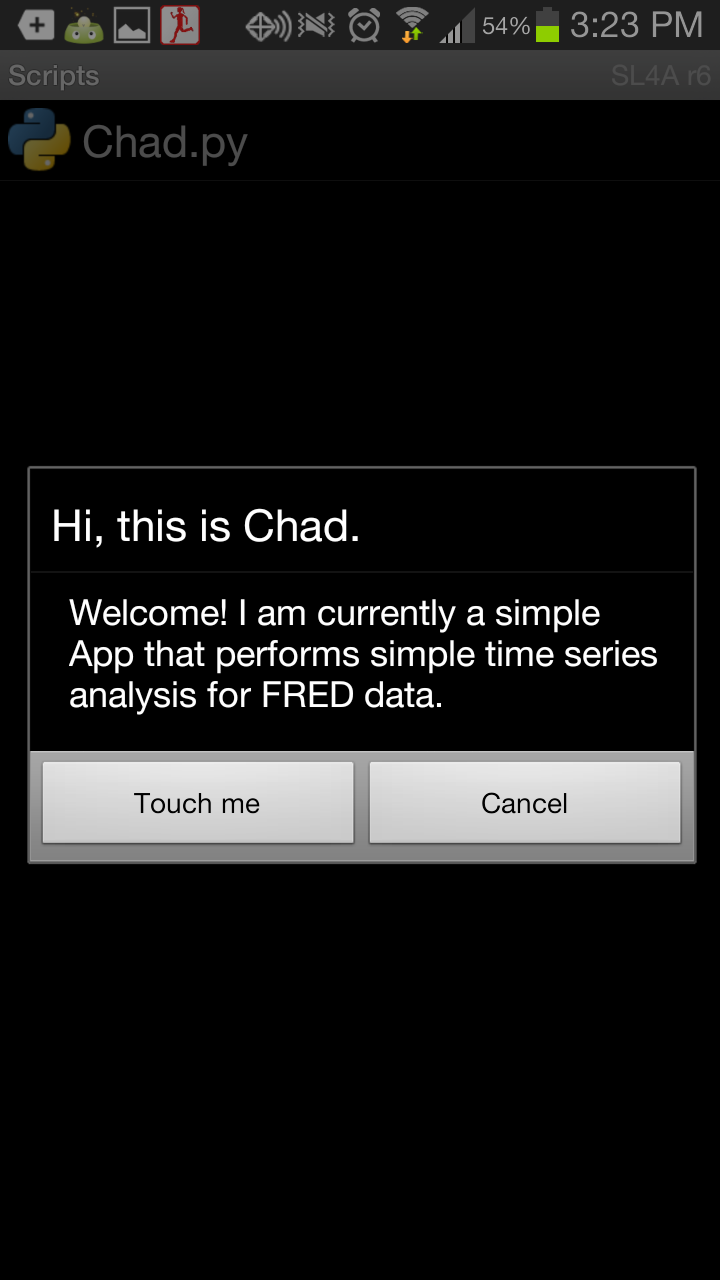
\includegraphics[clip=true,trim=0.2in 2.6in 0.4in 0.4in,scale=0.275]{greeting.png}}
\scalebox{0.6}{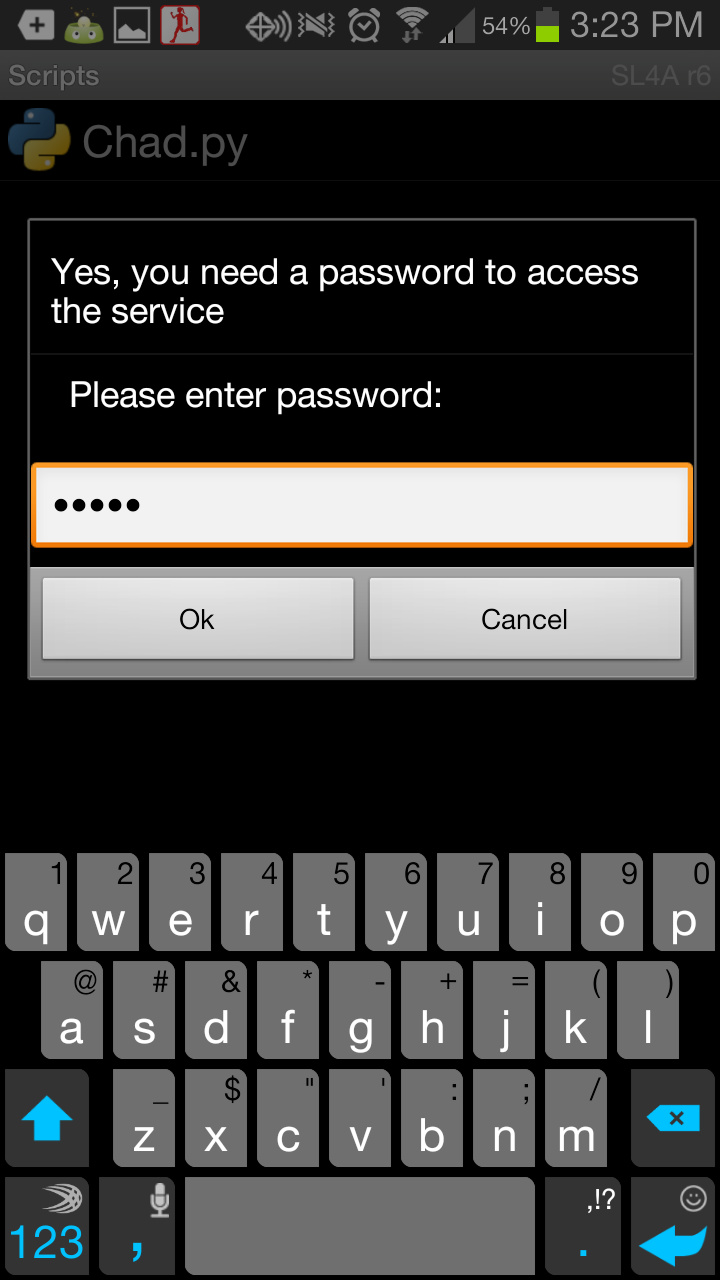
\includegraphics[clip=true,trim=0.2in 2.6in 0.4in 0.4in,scale=0.275]{enter_passcode.png}}
\scalebox{0.6}{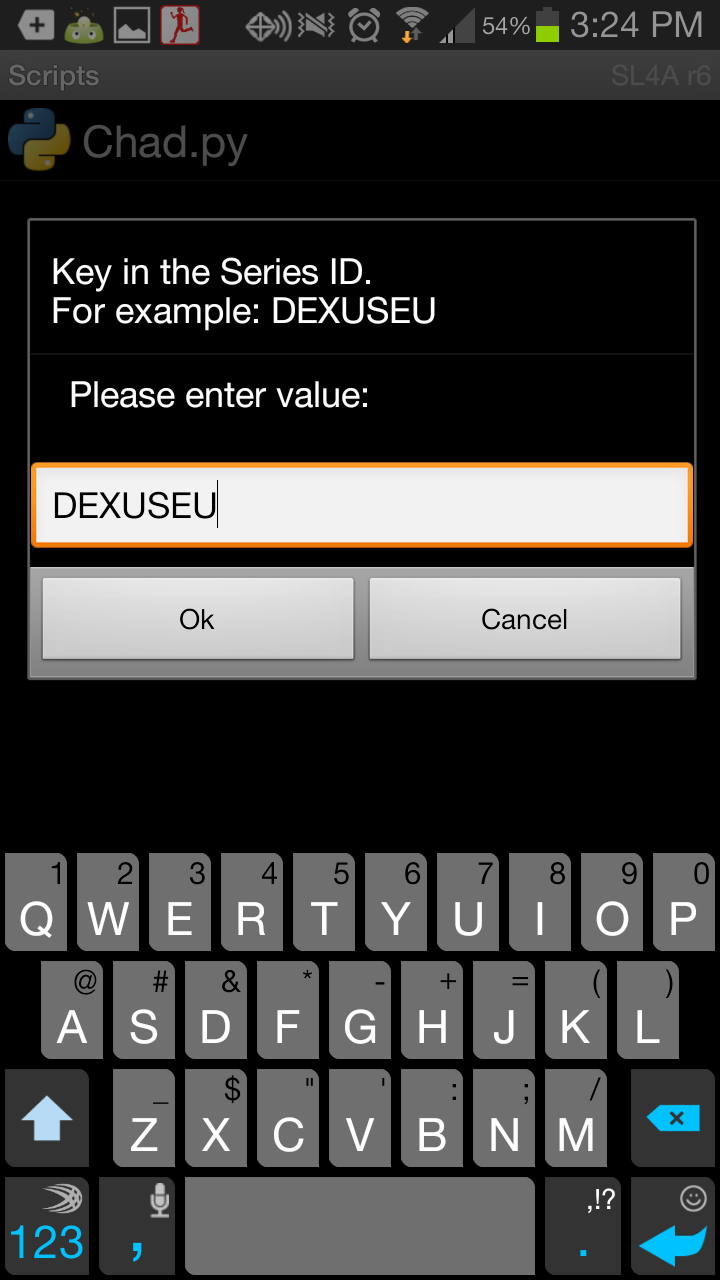
\includegraphics[clip=true,trim=0.2in 2.6in 0.4in 0.4in,scale=0.275]{enter_ticker.png}}

\caption{Screenshot of initial dialog-box that greets the user (left),
prompt the user to enter passcode to the program (middle),
allow user to enter the series ID of the data (right).In the future, it is possible to allow users to search for a specific dataset without knowing the exact series ID.}

\label{fig:initial screens}
\end{figure}

\begin{figure}[htb]
\centering

\scalebox{0.5}{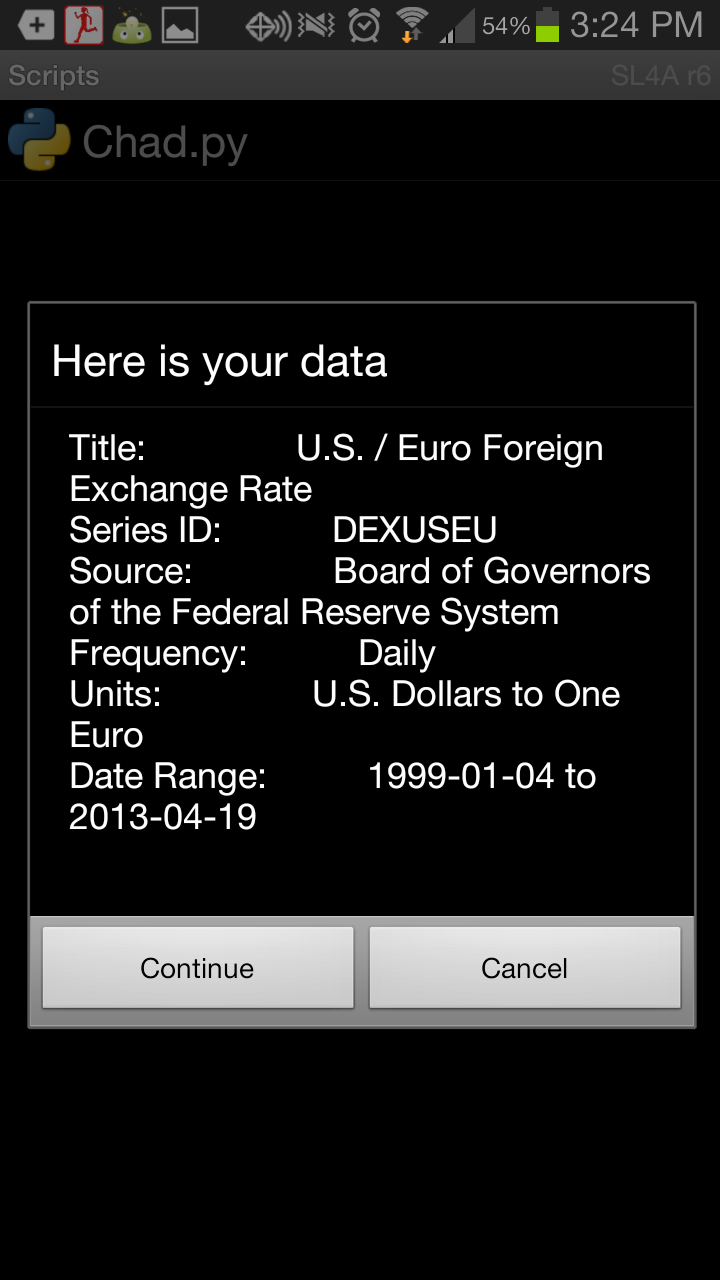
\includegraphics[clip=true,trim=0.2in 2.6in 0.4in 0.4in,scale=0.275]{data_info.png}}
\scalebox{0.5}{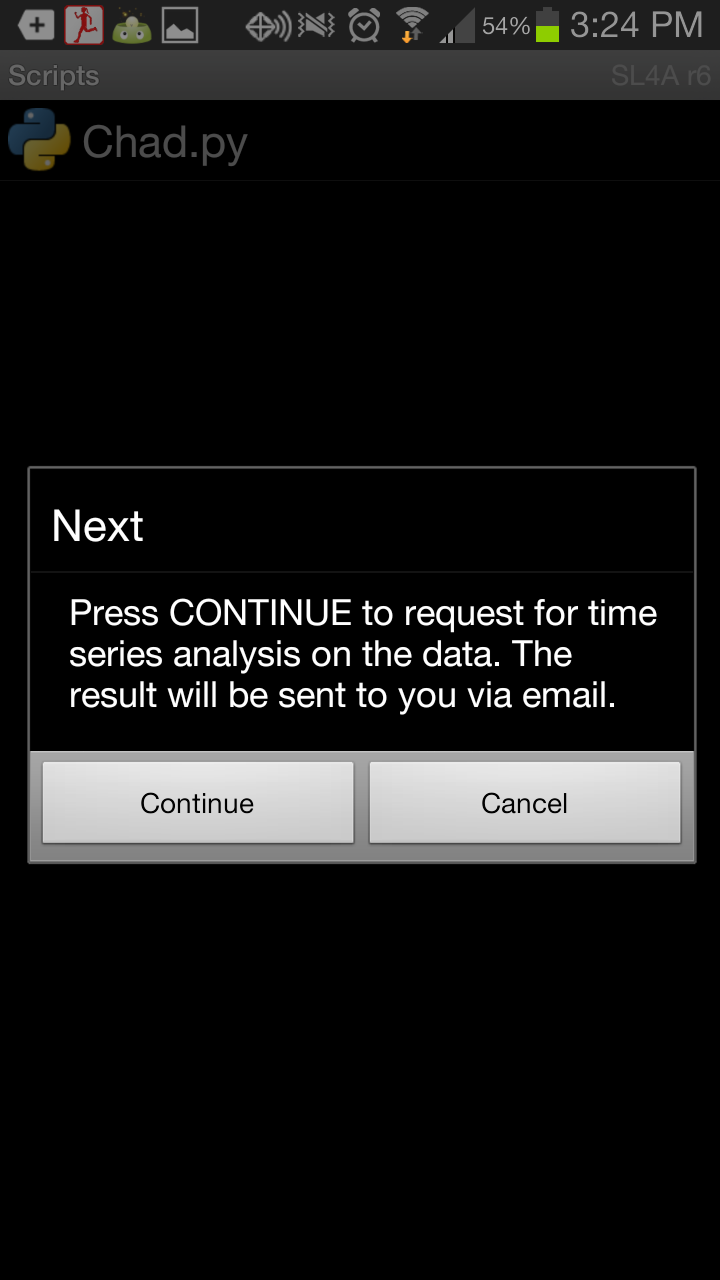
\includegraphics[clip=true,trim=0.2in 2.6in 0.4in 0.4in,scale=0.275]{email_alert.png}}
\scalebox{0.5}{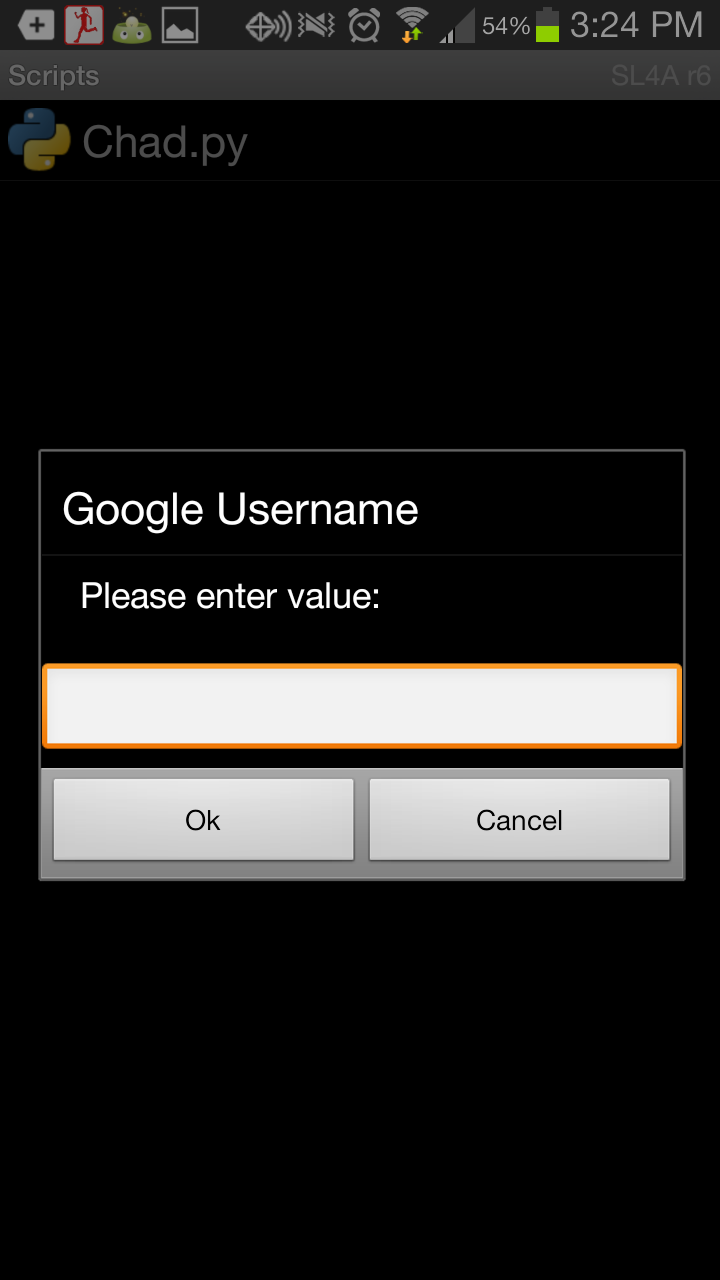
\includegraphics[clip=true,trim=0.2in 2.6in 0.4in 0.4in,scale=0.275]{google_user.png}}
\scalebox{0.5}{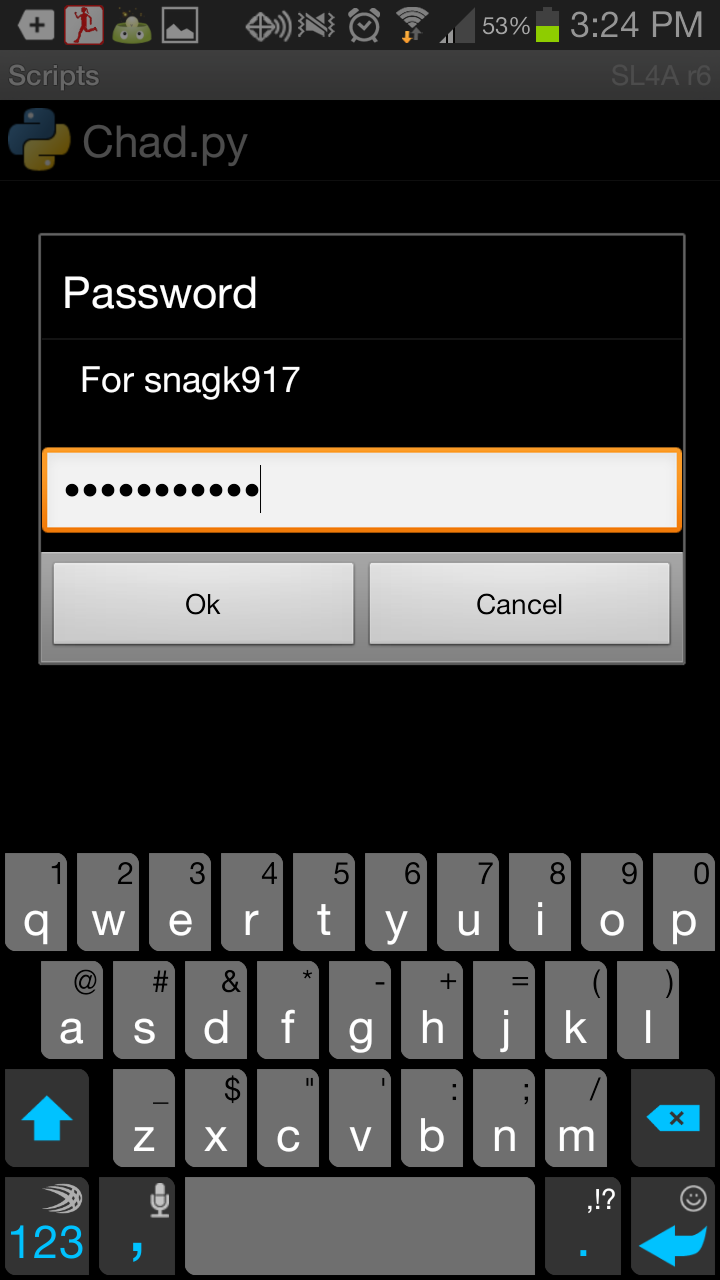
\includegraphics[clip=true,trim=0.2in 2.6in 0.4in 0.4in,scale=0.275]{google_password.png}}
%\includegraphics[width=0.15\textwidth]{images/corner-raw.jpg}
%\includegraphics[width=0.15\textwidth]{images/corner-ispink.jpg}
%\includegraphics[width=0.15\textwidth]{images/corner-ispink-binary.jpg}
%\includegraphics[width=0.15\textwidth]{images/corner-border-corners-cropped.jpg}
\caption{If it is the correct ID, the program will display the basic information about the dataset, this is the same information displayed on the FRED website (left);
Then it asks the user if data analysis is needed, press cancel will exit the program (middle);
If 'Continue' is pressed, the program prompt the user to enter his or her Gmail account information (right).}

\label{fig:data_info}
\end{figure}


\begin{figure}[htb]
\centering


\scalebox{0.6}{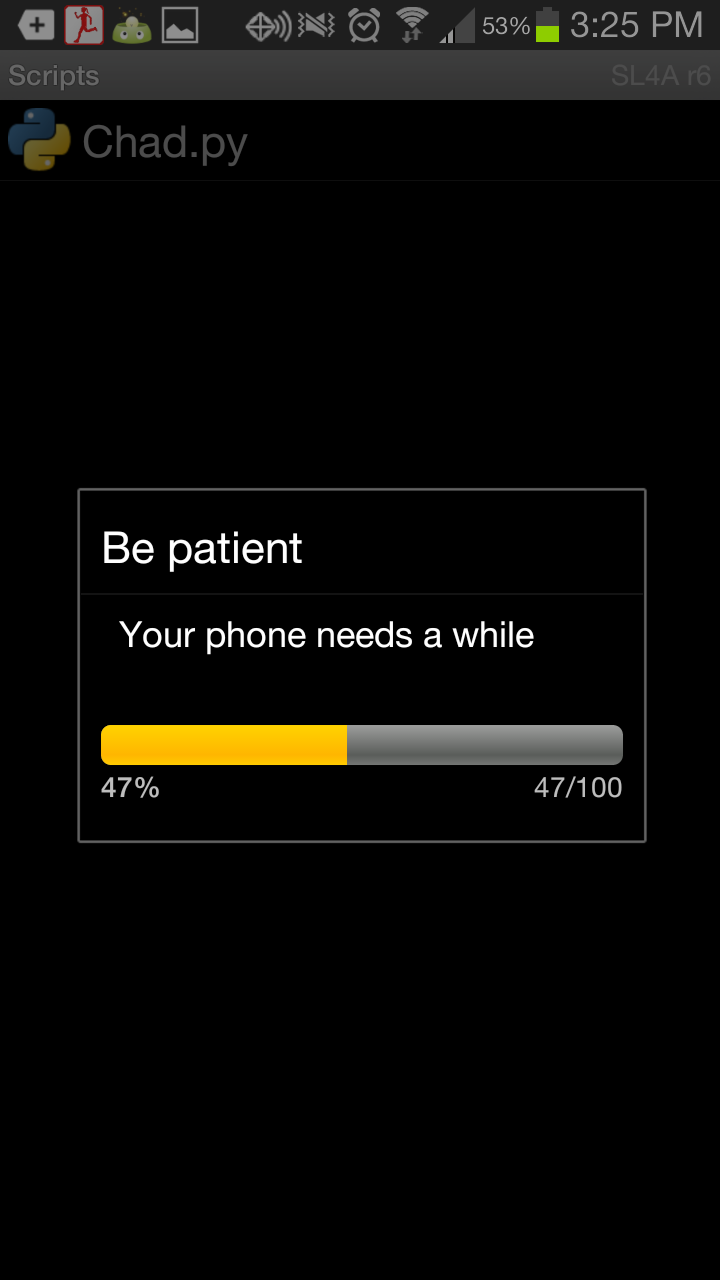
\includegraphics[clip=true,trim=0.2in 2.6in 0.4in 0.4in,scale=0.275]{progress.png}}
\scalebox{0.6}{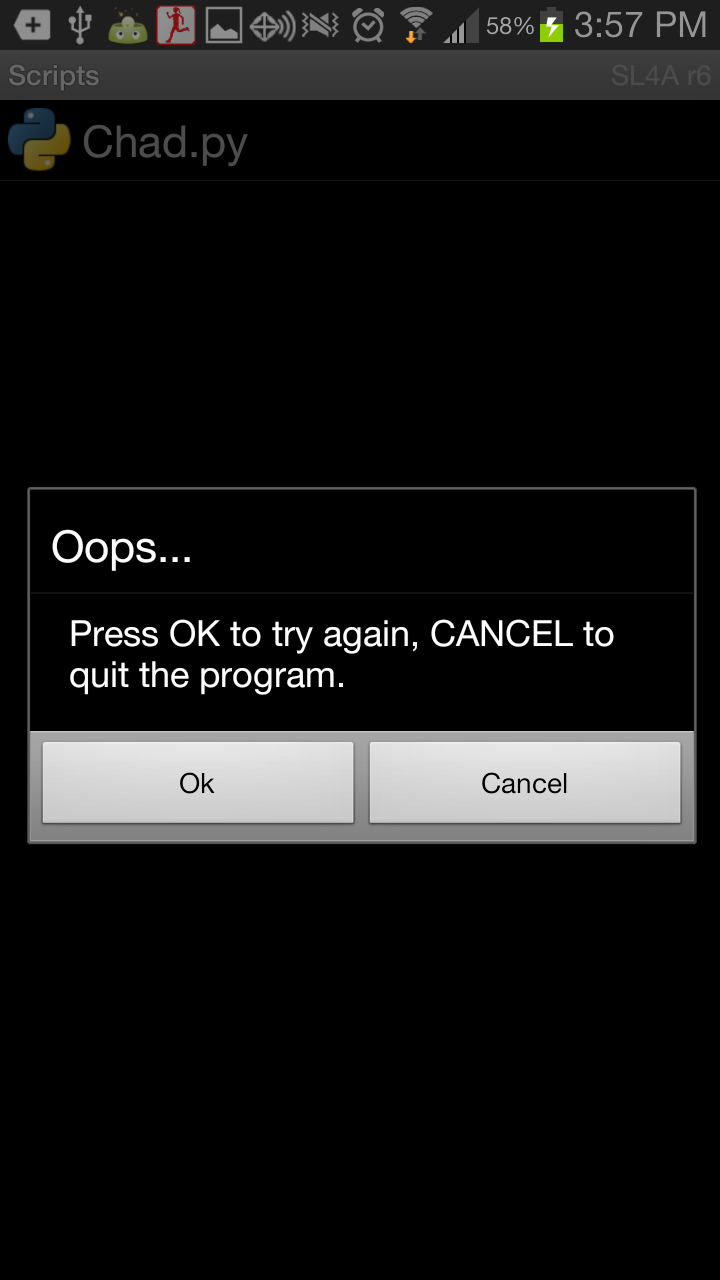
\includegraphics[clip=true,trim=0.2in 2.6in 0.4in 0.4in,scale=0.275]{oops.png}}
\scalebox{0.6}{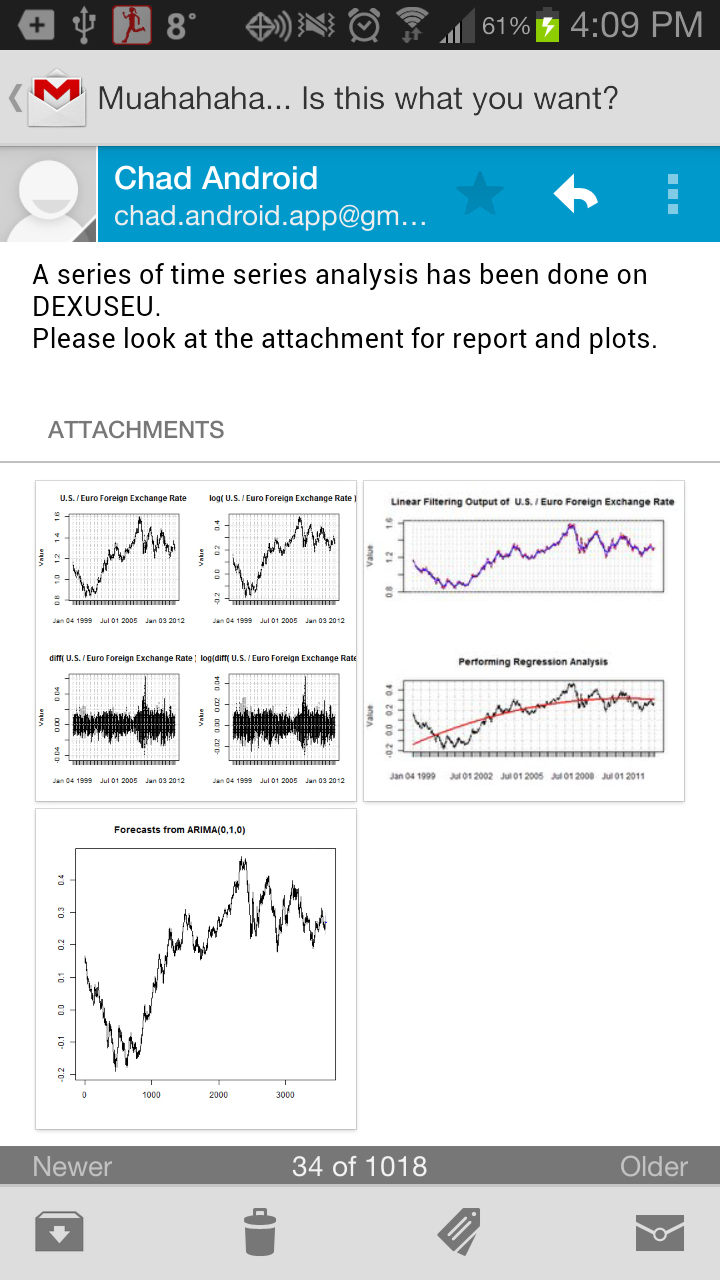
\includegraphics[clip=true,trim=0.2in 2.6in 0.4in 0.4in,scale=0.275]{result.png}}
%\includegraphics[width=0.15\textwidth]{images/corner-raw.jpg}
%\includegraphics[width=0.15\textwidth]{images/corner-ispink.jpg}
%\includegraphics[width=0.15\textwidth]{images/corner-ispink-binary.jpg}
%\includegraphics[width=0.15\textwidth]{images/corner-border-corners-cropped.jpg}
\caption{While sending the email, a progress bar pops out (left);
If there is any errors when keying in information, an error message pops out. If "Yes" is pressed, the program goes back and allow the user to try again. If same error is made too many times, the program tells the user and quit the program (middle);
In the end, the report is emailed back to the user (right).}

\label{fig:pink_classifier}
\end{figure}


This program has a lot of extensiable potential. With Python, it is very tedious to write a complete App GUI, as it requires writing HTML, Javascript and CSS from scratch. Java has a better support for these purposes. Also, the analysis can be tailored by the user to suit their needs.

\end{document}
